\clearpage
\subsection{Ultrasonic evaluation}
\begin{figure}
\centering
    \begin{subfigure}[b]{\picwidth}
        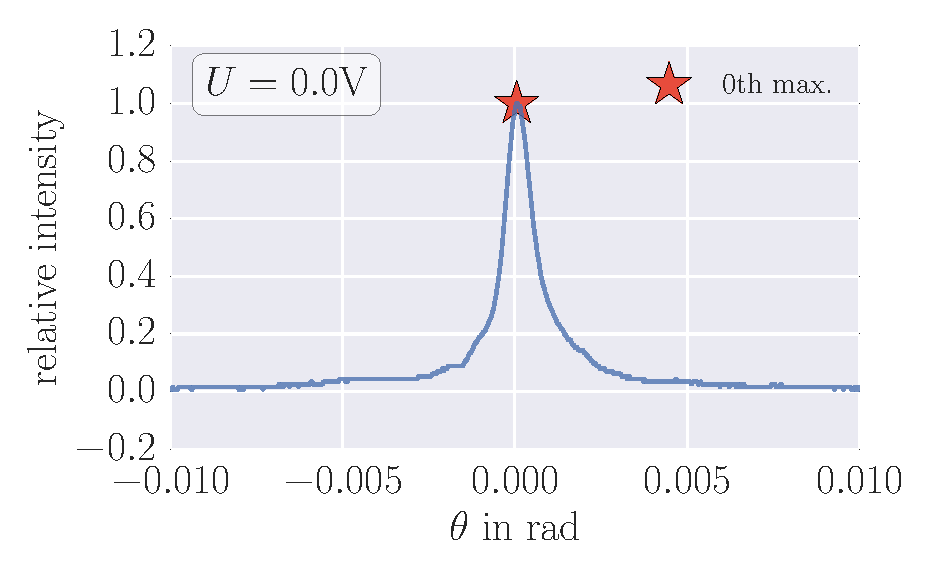
\includegraphics[width=1.0\textwidth]{analysis/figures/raman_001}
        \caption{}
        \label{fig:raman_001}
    \end{subfigure}
    \begin{subfigure}[b]{\picwidth}
        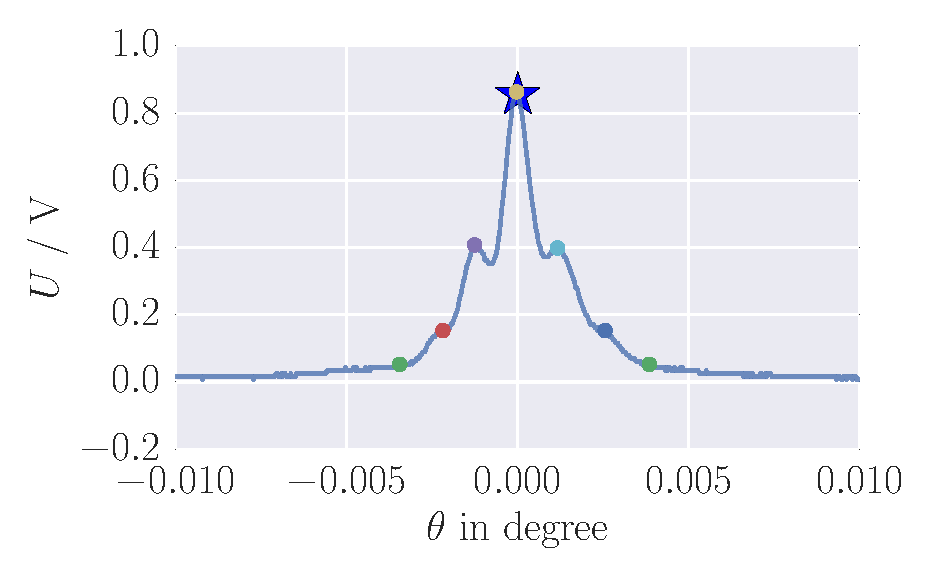
\includegraphics[width=1.0\textwidth]{analysis/figures/raman_007}
        \caption{}
        \label{fig:raman_007}
    \end{subfigure}
    \begin{subfigure}[b]{\picwidth}
        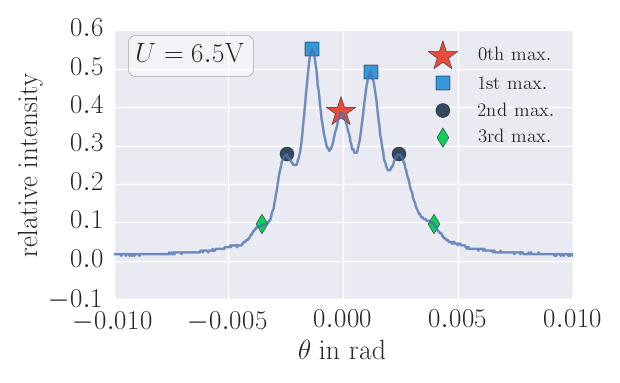
\includegraphics[width=1.0\textwidth]{analysis/figures/raman_014}
        \caption{}
        \label{fig:raman_014}
    \end{subfigure}
    \begin{subfigure}[b]{\picwidth}
        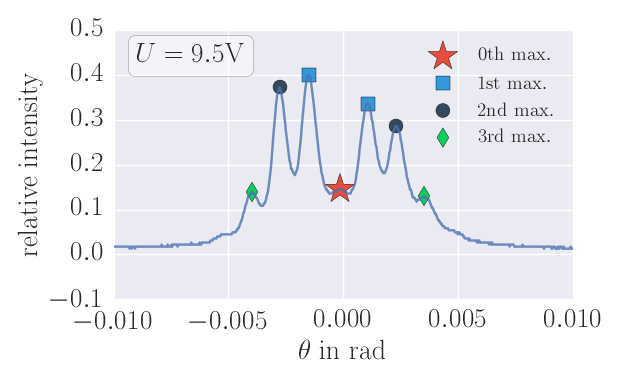
\includegraphics[width=1.0\textwidth]{analysis/figures/raman_020}
        \caption{}
        \label{fig:raman_020}
    \end{subfigure}
    \caption{A subsection of the data from the ultrasonic experiment.}\label{fig:raman}
\end{figure}
\begin{figure}[htpb]
    \centering
    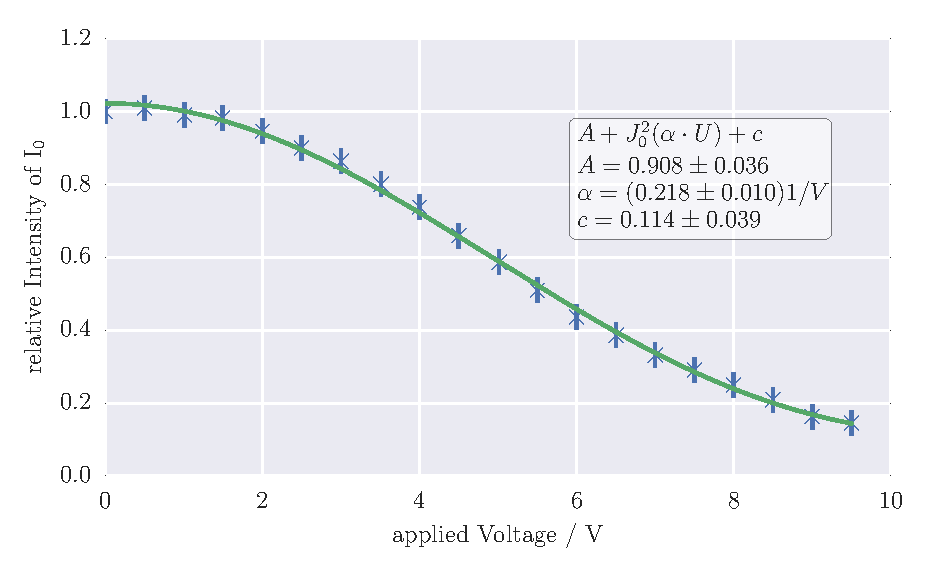
\includegraphics[width=1\textwidth]{analysis/figures/besselfit_0}
    \caption{This is the fit of the maxima of zeroth order. The error is given by 3\% of the extent of the oscilloscope.}
    \label{fig:besselfit_0}
\end{figure}


\begin{align}\Rightarrow \qquad
    \alpha &=& 0.218 \pm 0.010 \\
    A &=& 0.91 \pm 0.04 \\
    c &=& 0.11 \pm 0.04 
\end{align}


\begin{table}
    \centering
    \caption{covariance matrix}

 \begin{tabular}{|r|r|r|r|}
 \hline 
\cellcolor{tabcolor}&\cellcolor{tabcolor}$\alpha$&\cellcolor{tabcolor}$A$&\cellcolor{tabcolor}$c$\\ \hline 
 \cellcolor{tabcolor}$\alpha$&$0.00010$ &$-0.00029$ &$0.00037$ \\ \hline
\cellcolor{tabcolor}$A$&$-0.00029$ &$0.00136$ &$-0.00135$ \\ \hline
\cellcolor{tabcolor}$c$&$0.00037$ &$-0.00135$ &$0.00156$ \\ \hline
\end{tabular}
\end{table}
